% icstdoc.tex V1.11 11 April 2011
%brave new ideas, artistic installations with technological content, technical creative demonstrators
\documentclass[fonts]{icst}

\usepackage{moreverb}

\usepackage[breaklinks,colorlinks,bookmarksopen,bookmarksnumbered,linkcolor=ICSTblue,citecolor=ICSTblue,urlcolor=ICSTblue]{hyperref}
\usepackage{breakurl}
\usepackage{doi}
\usepackage{float}
\usepackage{graphicx}


\newcommand\BibTeX{{\rmfamily B\kern-.05em \textsc{i\kern-.025em b}\kern-.08em
T\kern-.1667em\lower.7ex\hbox{E}\kern-.125emX}}

\def\volumeyear{2014}

\begin{document}

\runningheads{Tomazic, Tomaz; Lai Chin Chung, Louis}{Trzaska cesta 25, 1000 Ljubljana}

\title{Virtual Skiing}

\author{Tomazic, Tomaz; Lai Chin Chung, Louis}

\address{University of Ljubljana, Faculty of informatics and computer science}

\abstract{This paper describes a virtual skiing game using kinect and unity 3D.}

\keywords{skiing, kincect, unity 3D, virtual}


\maketitle

\section{Introduction}
The interactive installation "Virtual skiing" enables a visual immersion into the feelings of gliding on snow through a winter landscape. The computer rendered winter landscape is displayed over the entire wall in front of the skier. As on real skis you can regulate the speed of descent by changing the posture of your body so that the air resistance is decreased or increased. By shifting the weight of your body to the right or left ski you can make turns down the slope between the snow capped trees. The interface to the virtual world is implemented by computer vision techniques which capture the posture of the skier's body. \cite{ORIG}).

\section{Software overview}
\subsection{Goal of the project}
The goal of the project is to provide the user a virtual skiing experience. To do so, at least the following needs to be done:
\begin{enumerate}
\item[(i)] track body movement of the user
\item[(ii)] display a virtual 3D environment on a screen
\item[(iii)] play game in this enviroment
\end{enumerate}


\subsection{Kinect}
\subsubsection{Overview}
Kinect is the most convienent body movement tracking hardware we can find in the market, it thus becomes the tool for our project. The Kinect sensor haveo one RGB camera and two Infra-red sensors, allowing it to track movement to/from any direction in a 3D space. 

\subsubsection{Code}
By examining the sample code, a skeleton of user is made using C\#. A skeleton consist of nodes and lines, nodes representing the the joints of the user, lines representing the limbs/body of the user. By comparing the positions nodes, we can capture the user's movement and turn them into inputs in the game.There are 2 main types of input in the skiing game, one controls the direction and the other controls the speed of skiing.

\subsubsection{Directions}
To control the direction of ski, user need to band their body left or right to turn, or stay in the middle to go straight. A simple method is used to extract this particular movement by the user, we simply compare the nodes on both shoulders. The data obtained is then threasholded into only 3 inputs, left, middle and right. 

\subsubsection{Speed}
The user need to squat to increase the speed, and detection of squatting is needed. When squatting, the position of the node on hip is changing obviously. So, the node on hip is used to determine whether the user is squatting or not.


\section{Developing process}
\subsection{Planning}
\subsubsection{Mindmap}
A mindmap is made to record all the ideas about the project. It gives the team some guide and direction to work on. This is also the step where we know each team member's strength and weakness, leads to better allocation of work later on. 

\begin{figure}
    \centering
    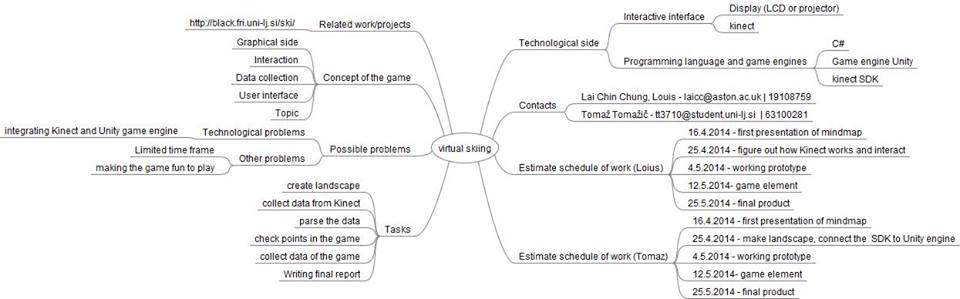
\includegraphics[width=0.4\textwidth]{mindmap.png}
    \caption{Mindmap}
    \label{fig:awesome_image}
\end{figure}

\subsection{Research}
At the beginning of the project, none of the team member knows anything about programming on Kinect, it is the main focus of search. We found that Kinect SDK is essential in coding the sensor, it comes together with Kinect studio and a developer toolkit. Kinect studio is just for testing and the developer toolkit is a package of code examples.

For the displaying of the virtual skiing world, it took us almost no time to search for game engine, one of the team member knows how to use Unity 3D, certainly this becomes your choice of game engine. 

\subsection{Divide the work}
The work of the project can be divided into two main parts, the input(Kinect) and output(the display). Chin Chung will work on Kinect, figure out how it works; Tomaz will work on the game engine, create a virtual 3D world for the user to ski on. 

\subsection{Unity}
Unity is a development engine for the creation of 2D and 3D games and interactive content. It has multiplatform support and own asset store where you can download scripts, objects, scenes.. \cite{UNITY}
We found kinect wrapper package\cite{MERGE} for Unity3D engine, which added us easy option to get collected data from kinect directly to our script code in unity. We used this data to calculate angle between different joints. With this angle we are then able to set intensity of turning sensitivity. To gamify our enviroment we put score counter in top left corner, which get increased by colliding carracter with advertised flags on the way down. To allow kinect detecting the human body and give user time to prepare we put countdown at the beginning of game.

\begin{figure}
    \centering
    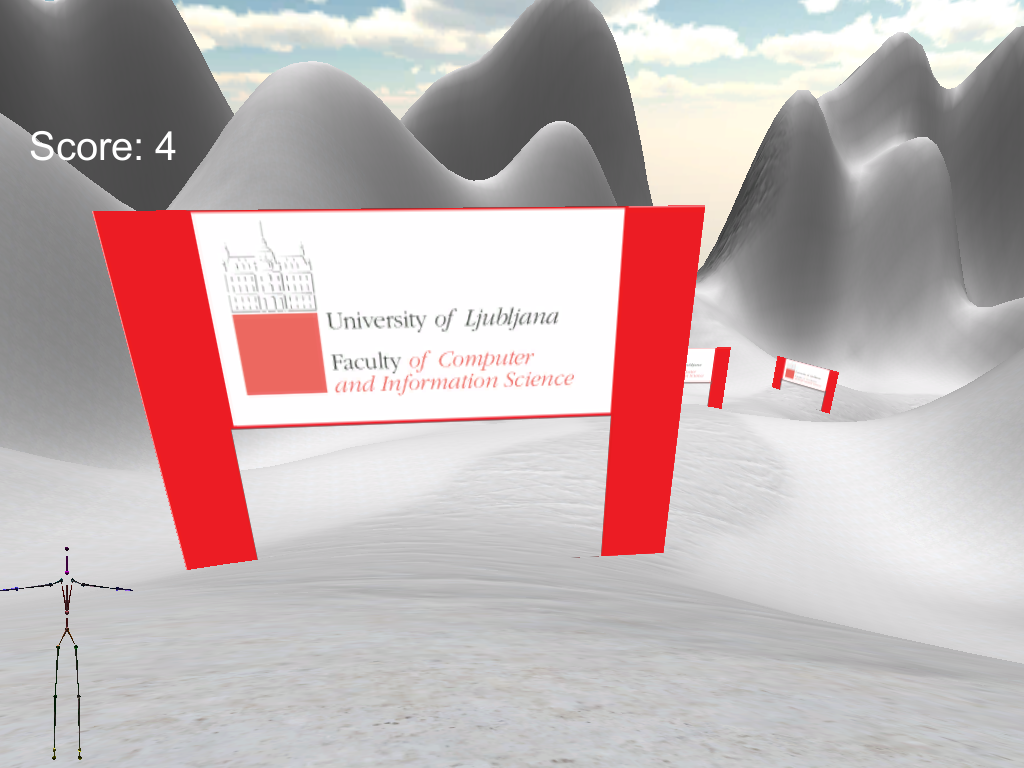
\includegraphics[width=0.4\textwidth]{game.png}
    \caption{Screenshot form skiing game.}
    \label{fig:awesome_image}
\end{figure}

\subsubsection{Terrain}
It has great support for creating terrain. In game we created simple terrain with mountains and put snow on it. For more flexible terrain we could create scirpt or just few images of pre-difined heightmaps. Unity have option to generate terrain using hightmap.

\subsubsection{Scripting}
Unity support C\#, javascript and Boo scripting languages. It also supports applying different languaged script on same object. We used such ability for user movement in skiing game, using javascript and C\# languages only.




\subsection{Kinect}
The first attemt to work on Kinect was a failure, not until I start working on it, I didn't notice the underlying problems. I did get the skeleton of the user, retrieving some data from it, but they are not very useful. I faced three main problems in this part. 

\subsubsection{C\#}
I did learn several languages before, but not C\#. When I read the code, I understand them in a very low level, I recognize almost all the syntex, the loops, conditionals, declarations... etc. It took me really a lot of time to get to a higher level of understanding. The documentations from Microsoft was not very useful, it maybe enough for an experienced C\# programmer, not for me.

\subsubsection{Mathematics}
fter a lot of reading, I finally locate the part where the orientation of the nodes/joints are stored. The orientations of the nodes are expressed in rotation quaternions , an absolutely alien term for me. I checked the documentation, wikipedia and other sites, they all explain it is a very mathematical way. The main direction I studied is software engineering, the mathematics they are using are far beyond my level. I just leave the output in the form of rotation quaternion.

\subsubsection{Developing evniroment}
I used the Microsoft visual studio in the part, mainly because most tutorials on Kinect are also on this environment. Problem comes when my part needs to merge with the game engine, I have no idea how to do it. Just importing the scripts in visual studio was not enough, the scripts will not run automatically. Scripts need to link to game objects in order to get running. Also the displaying machanism is very different in Visual Studio and Unity 3D, I don't know how to translate the code.

\subsection{Rework}
A replan is needed because the Kinect part and the Unity 3D part of the project was not mergeable. Another research is done to find Kinect code example directly in Unity 3D, not in Visual Studio. 

\subsubsection{Kinect in Unity 3D}
Code example was found in Unity 3D wiki, this time the whole Kinect part is coded only in the game engine. Work done in Visual Studio is repeated in Unity 3D, it was a lot smoother than before because of the experience gained. Instead of the rotational quaternion, a simpular axis system is used to compare the postions of the Joints. 

\subsubsection{C\# and Javascript}
The code is until not fully compatable, the graphics part uses Javascript and the Kinect part uses C\#. A way to transfer data between scripts in two langauges is found, and the problem is fully solved.


\section{Conclusions}
We were able to make game playable by setting correct parameters such as speed, turning speed, gliding and gravity accelleration. Project has been succesfully finished and requirements has been fullfield.

\begin{thebibliography}{9}

\bibitem{ORIG} \textsc{Solina Franc} and \textsc{Batagelj Borut} (2005) \emph{http://black.fri.uni-lj.si/ski/}

\bibitem{UNITY} \textsc{Unity 3D} (2014) \emph{\url{http://docs.unity3d.com/ScriptReference/index.html}}

\bibitem{MERGE} \textsc{Microsoft SDK} \emph{\url{http://wiki.etc.cmu.edu/unity3d/index.php/Microsoft_Kinect_-_Microsoft_SDK}}

\end{thebibliography}
\end{document}
